\PassOptionsToPackage{table,usenames,dvipsnames,x11names}{xcolor}
\documentclass[english,serif,mathserif]{beamer}
\usetheme[informal]{gc3}

\usepackage[T1]{fontenc}
\usepackage[utf8]{inputenc}
\usepackage{babel}

\usepackage{gc3}


\begin{document}


\title[Spark]{An Insufficient Introduction to Spark}
\subtitle{Part 1: The MapReduce computing model}
\author{Riccardo Murri \texttt{<riccardo.murri@gmail.com>}}
\date{2019-02-11}

%% Makes the title slide
\maketitle

%\part{Introduction}

\begin{frame}
  \frametitle{What is Spark?}

  \begin{center}
    \href{http://spark.apache.org}{Apache Spark}
    is a general-purpose \\
    distributed computation framework.
  \end{center}
\end{frame}


\begin{frame}[fragile]
  \frametitle{Parallel computing}
  ``In the simplest sense, \alert<1>{parallel computing is the simultaneous use
    of multiple compute resources} to solve a computational problem:

  \uncover<2>{%
    \begin{itemize}
    \item A problem is broken into discrete parts that can be solved concurrently
    \item \alert<2>{Instructions from each part execute simultaneously on different processors}
    \item {An overall control/coordination mechanism is employed}''
    \end{itemize}
  }%

  \+
  \begin{references}
    {\em Introduction to Parallel Computing}, \\
    Blaise Barney, Lawrence Livermore National Laboratory, \\
    \url{https://computing.llnl.gov/tutorials/parallel_comp/#Whatis}
  \end{references}
\end{frame}


\begin{frame}
  \frametitle{Distributed computing}

  ``A distributed system is a model in which components located on networked
  computers communicate and coordinate their actions by passing messages.

  \+
  \emph{[\ldots]}

  \+
  Three significant characteristics of distributed systems are:
  \begin{itemize}
  \item concurrency of components,
  \item lack of a global clock, and
  \item independent failure of components.''\note{%
      “A distributed system is one in which the failure of a computer
      you didn't even know existed can render your own computer
      unusable” -- Leslie Lamport
    }%
  \end{itemize}

  \+
  \begin{references}
    \url{https://en.wikipedia.org/wiki/Distributed_computing}
  \end{references}
\end{frame}


\begin{frame}
  \frametitle{Why distributed computing?}

  \begin{center}
    {\Large Scale out}
    \\
    Attack larger problems \\ by using multiple computers.

    \+\+
    {\Large Speed}
    \\
    Solve independent parts \\ of a problem concurrently.
  \end{center}
\end{frame}


\begin{frame}
  \frametitle{What's so hard about distributed computation?}

  \begin{itemize}
  \item \alert<1>{Synchronization:} Tasks need to be
    coordinated between the different machines.

    \+\item \alert<1>{Distributing} and
    \alert<1>{collecting} data across multiple processors can
    be verbose and complicated.

    \+\item No longer have one machine but many; \\
    \emph{hence}, \alert<1>{hard to debug} and prone to failures.
  \end{itemize}
\end{frame}


% \begin{frame}
%   \frametitle{What's so hard about distributed computation?}

%   General multiprocessing libraries (e.g. threads):
%   \begin{itemize}
%   \item give users a lot of control and flexibility;
%   \item can be hard to use and debug;
%   \item too low-level for quick development and testing of home-grown code!
%   \end{itemize}
% \end{frame}


\begin{frame}
  \frametitle{Liberation through limitation}

  Popular ``framework'' approach (Map/Reduce, BSP):
  \begin{itemize}
  \item \emph{Limited to a specific model of parallel computation}
    \begin{itemize}
    \item Users need/can only supply a few ``functions'' in a pre-determined scheme.
    \end{itemize}

  \item \emph{Framework takes cares of work+data distribution and fault-tolerance}
  \end{itemize}

  \+
  Usefulness of a framework depends on how broad a class of problems
  the parallel computing model can be applied to.
\end{frame}


\part{MapReduce}

\begin{frame}[fragile]
  \small
  Let's start with some concrete examples.

  \+
  \begin{exercise*}[1.A]
    Write a function \texttt{Lengths(L)} that takes a list \texttt{L} of
    \emph{strings} and returns a list of the their lengths.
  \end{exercise*}

  \+
  \begin{exercise*}[1.B]
    Write a function \texttt{LongerThan(L, m)} that takes a list
    \texttt{L} of strings and a single value \texttt{m}, then returns
    a list of those strings in \texttt{L} whose length is larger than
    \texttt{m}.
  \end{exercise*}

  \+
  \begin{exercise*}[1.C]
    Write a function \texttt{Sum(L)} that takes a list \texttt{L} of numbers and
    returns the sum of all of them.
  \end{exercise*}

  \+
  \begin{exercise*}[1.D]
    Write a function \texttt{RandList(N)} that takes generates and
    returns a list of \texttt{N} random floating-point numbers (each
    ranging from \texttt{0.0} to \texttt{1.0}).
  \end{exercise*}

\end{frame}


\begin{frame}
  \frametitle{map, reduce, filter (1)}

  Constructing a new list by looping over a given list and applying a function
  on all elements is \emph{so common} that there are specialized functions for that:

  \+
  \begin{describe}{map(fn, L)}
    Return a new list formed by applying function \texttt{fn(x)} to every
    element \texttt{x} of list \texttt{L}
  \end{describe}

  \+
  \begin{describe}{reduce(fn2, L)}
    Apply \emph{associative} function \texttt{fn2(x,y)} to the first two items \texttt{x} and
    \texttt{y} of list \texttt{L}, then apply \texttt{fn2} to the result and the
    third element of \texttt{L}, and so on until all elements have been
    processed --- return the final result.
  \end{describe}
\end{frame}


\begin{frame}
  \frametitle{map, reduce, filter (2)}

  \begin{describe}{filter(fn, L)}
    Return a new list formed by elements \texttt{x} of list \texttt{L} for which
    \texttt{fn(x)} evaluates to a ``True'' value.
  \end{describe}

  \+
  \begin{seealso}
    \url{http://www.python-course.eu/lambda.php}
    and \url{https://docs.python.org/3/howto/functional.html} (more advanced)
  \end{seealso}
\end{frame}


\begin{frame}[fragile]
  This is how you could rewrite the examples \\
  using \texttt{map}, \texttt{reduce}, and \texttt{filter}.

  \begin{columns}
\begin{column}{0.5\linewidth}
\begin{python}
# *** ex 1.A ***
def Lengths(S):
  return map(len, S)

# *** ex 1.C ***
def Sum(L):
  from operator import add
  return reduce(add, L)
\end{python}
\end{column}
    \begin{column}{0.5\linewidth}
\begin{python}
# *** ex 1.B ***
def LargerThan(L, m):
  # note: can define
  # func's in func's!
  def good(s):
    return (len(s) > m)
  return filter(good, L)
\end{python}
\end{column}
  \end{columns}
\end{frame}


\begin{frame}
  \begin{exercise*}[1.E]
    A rough approximation to the constant $\pi$ can be computed (using
    a Monte Carlo method) as follows:
    \begin{enumerate}
    \item Let $N>0$ be a large integer,
    \item pick $N$ points in the square $\{(x,y): 0 < x, y < 1 \}$ uniformly at random;
    \item count the number $P$ of points that fall into the unit circle $\{(x,y): x^2 + y^2 < 1 \}$;
    \item for large enough $N$, the ratio $P/N$ approximates the area of a quarter of the unit circle, i.e. $\pi/4$.
    \end{enumerate}
    Write Python code that computes an approximation to $\pi$ using the above procedure.
  \end{exercise*}
\end{frame}


\begin{frame}
  \begin{center}
    {\huge
      What is the advantage of \\
      \texttt{map}+\texttt{reduce} over loops?}

    \+
    \only<2>{%
      \Huge
      \alert<2>{Parallelism.}
    }
  \end{center}
\end{frame}


\begin{frame}
  \frametitle{MapReduce: advantages of the model}
  \begin{quote}
    ``Programs written in this style \\ are \emph{automatically
      parallelized} \\ and executed on a large cluster of machines''
  \end{quote}

  \+
  \begin{references}
    Dean and Ghemawat, \\
    \href{http://research.google.com/archive/mapreduce.html}{MapReduce:
      Simplified Data Processing on Large Clusters}
  \end{references}
\end{frame}


\begin{frame}
  \frametitle{{\color{red}Map}Reduce}

  \begin{columns}
    \begin{column}{0.33\textwidth}
      \uncover<1>{%
      The {\color{red}Map} function processes a key/value pair to
      produce intermediate key/value pairs.
      }%

      \+\+

      \uncover<2>{%
        The {\color{blue}Reduce} function  merges all intermediate values
        associated with a given key.
      }%
    \end{column}
    \begin{column}{0.66\textwidth}
      \+
      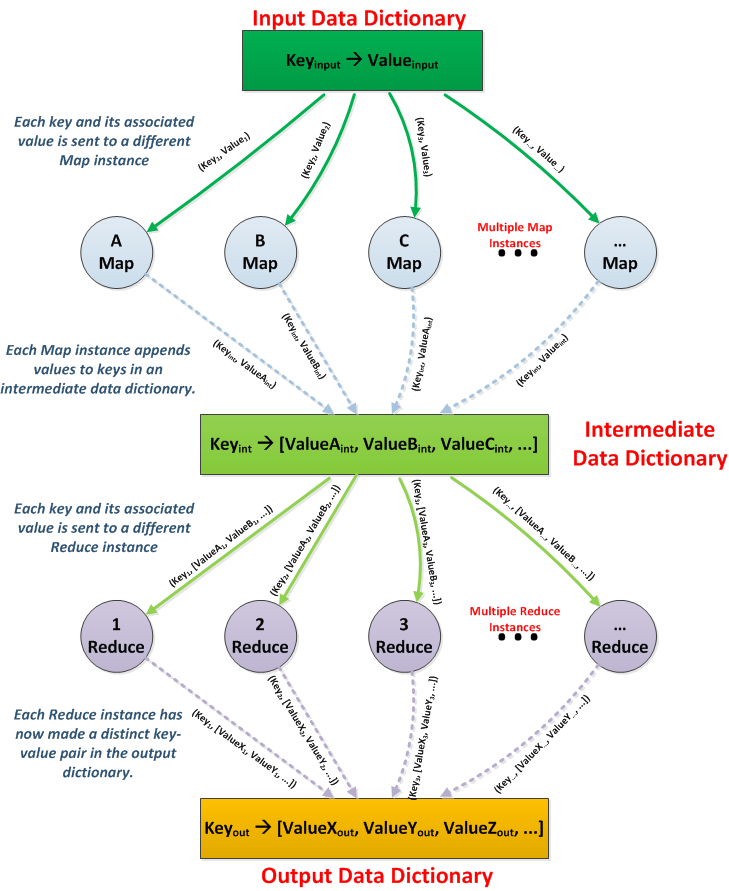
\includegraphics[clip,width=0.9\linewidth]{fig/MapReduce}
    \end{column}
  \end{columns}

  \+\+\+
  {\tiny\em
    Image source: Greiner, J., Wong, S.:
    \href{http://www.clear.rice.edu/comp130/12spring/MapReduce/}{Distributed Parallel Processing with MapReduce}}
\end{frame}


\begin{frame}[fragile]
  \frametitle{Example: word count}
  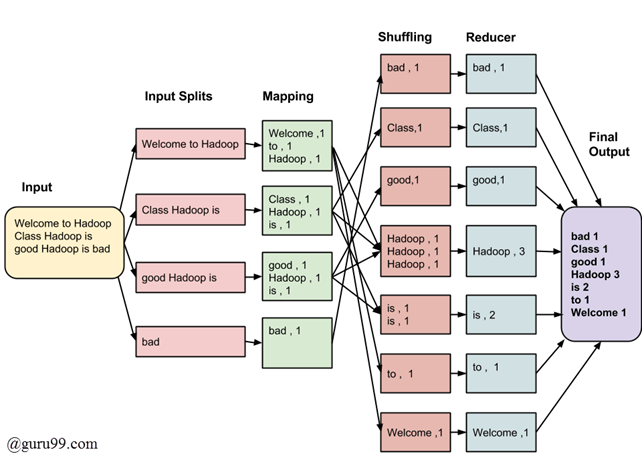
\includegraphics[width=0.8\textwidth]{fig/mr-pipeline}

  \small
  \only<1>{
    \+
    Input is a text file, to be \emph{split} at line boundaries.
  }
  \only<2>{
    \+
    The \emph{Map} function scans an input line and outputs a pair
    \emph{(word, 1)} for each word in the text line.
  }
  \only<3>{
    \+
    The pairs are \emph{shuffled} and sorted so that each reducer gets
    all pairs \emph{(word, 1)} with the same \emph{word} part.
  }
  \only<4>{
    \+ \small
    The \emph{Reduce} function gets all pairs \emph{(word, 1)} with
    the same \emph{word} part, and outputs a single pair \emph{(word,
      count)} where \emph{count} is the number of input items received.
  }
  \only<5>{
    \+ \small
    The global output is a list of pairs \emph{(word, count)} where
    \emph{count} is the number of occurences of \emph{word} in the input
    text.
  }

  \+
  \only<1>{\tiny\em Image source: \url{http://www.guru99.com/introduction-to-mapreduce.html}}
\end{frame}


\begin{frame}
  \frametitle{MapReduce: features of the implementation}
  \begin{quote}
    The run-time system takes care of the details:
    \begin{itemize}
    \item<2-> partitioning the input data,
    \item<3-> scheduling the program execution,
    \item<4-> handling machine failures,
    \item<5-> managing the required inter-machine communication.
    \end{itemize}
  \end{quote}

    \+
    These are all \emph{highly nontrivial} tasks to handle!

  \+
  \only<-5>{%
    \begin{references}
      Dean and Ghemawat: \\
      \href{http://research.google.com/archive/mapreduce.html}{MapReduce:
        Simplified Data Processing on Large Clusters}
    \end{references}
    }%
\end{frame}


\begin{frame}
  \frametitle{What MapReduce is {\em not} good for}

  Low-latency computation \\ (e.g., interactive tasks).
  \\

  \+
  \begin{flushright}
    Iterative computation \\ (no provision to re-use \\ already-computed
    results)
  \end{flushright}

  \+
  Problems which cannot easily \\ be partitioned or~recombined \\ (i.e., do
  not fit the paradigm)
\end{frame}


\part{Appendix}
\begin{frame}
  \frametitle{References}

  Dean, J., and Ghemawat, S.:
  \href{http://research.google.com/archive/mapreduce.html}{``MapReduce: Simplified Data Processing on Large Clusters''},
  OSDI'04

  \+
  Greiner, J. and Wong, S.:
  \href{http://www.clear.rice.edu/comp130/12spring/MapReduce/}{``Distributed Parallel Processing with MapReduce''}

%   \+
%   Roškar~R.: ``\,`Big' Data analysis using Apache Spark'',
%   \url{https://github.com/rokroskar/spark_workshop}
\end{frame}


\end{document}

%%% Local Variables:
%%% mode: latex
%%% TeX-master: t
%%% End:
